\documentclass{article}
\usepackage[utf8]{inputenc}
\usepackage{graphicx}
\usepackage[margin=1in]{geometry}
\title{Beam Geometries and their Strength}
\author{Matthew Zhang}
\date{June 2018}

\begin{document}

\maketitle


\section*{Abstract}
\quad 
This experiment was conducted in order to answer a question concerning torques and forces: How do well do different shapes of beams resist bending due to a load being placed on their end? In class the concept of torques had already been introduced as a type of "rotational force". The experiment tested 3D-printed beams of various different profiles by hanging weights off of their ends when supported cantilever on one end. This experiment subjected various objects to a constant torque and examined how they performed mechanically due to the torque. The experiment found that profiles containing more material tended to perform better, with an increased effectiveness if the material is located in the dimension of the load.



\section*{Procedure}
\textbf{Materials:}\newline
3D-Printed beams\newline
String\newline
Clamp\newline
Digital Caliper\newline
Two 200g Weights\newline
Balance Scale\newline
\newline
\textbf{Independent Variables:}\newline
Beam Shape \newline
Beam Mass \newline
\newline
\textbf{Dependent Variables:}\newline
Displacement of beam end\newline
\newline
\textbf{Data Collection:}\newline
\begin{enumerate}
\item 
Take a beam and clamp it to the table, making sure that the end hangs off 85 mm off of the edge of the table. Orient it so that the hole in the beam goes sideways, and is also hanging off the table
\item
Tie a string around the hole in the beam and attach two 200g weights to the end of the string
\item
Place a meter stick next to the bending beam to use as a horizontal reference, and measure the amount of bending by using the caliper to measure dimension along the vertical axis from the top of the meterstick to the bottom of the end of the beam
Record this value
\item
Use a scale to measure the mass of the beam
\item
Repeat steps 1-4 for every single beam
\item
Measure and record the height of the meterstick
\end{enumerate}
\textbf{Diagram:}\newline
\begin{center}
	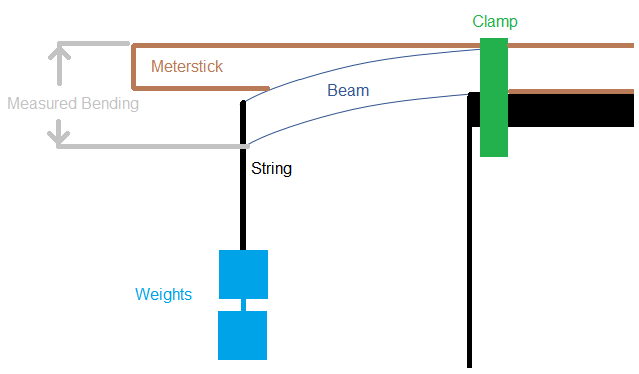
\includegraphics[width=.8\linewidth]{whysicDiagram.png}
\end{center}
\textbf{Shapes:}\newline
\begin{center}
	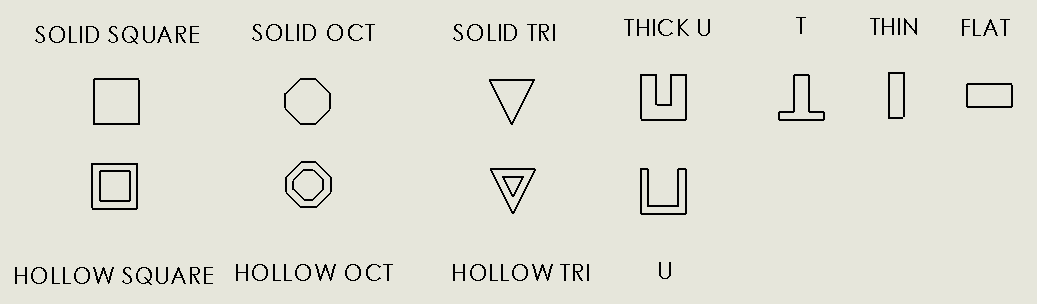
\includegraphics[width=.8\linewidth]{Shapes.png}
\end{center}
\pagebreak
\section*{Data}
\textbf{Data Table:}\newline
\begin{center}
	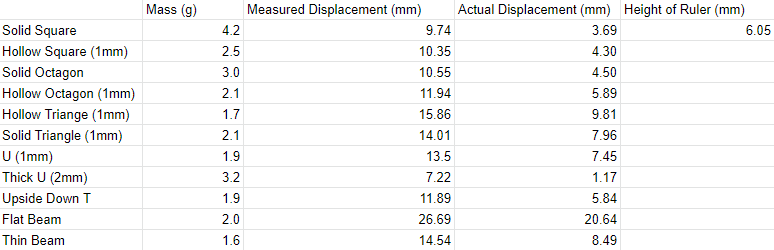
\includegraphics[width=.8\linewidth]{Table.png}
\end{center}
\textbf{Data Chart:}\newline
\begin{center}
	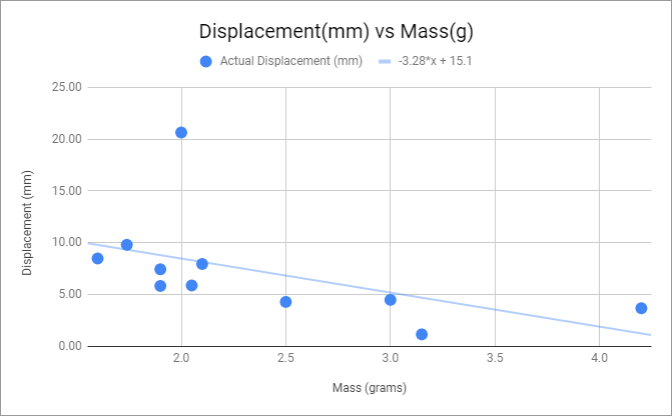
\includegraphics[width=.8\linewidth]{Chart.png}
\end{center}
\quad 
The data appears to be somewhat linear, with a notable outlier being the "flat" beam, which had a much greater displacement. Overall, the trend is that beams of greater mass will most likely deflect less. However, as the shape of the graph is not exactly linear, and because the outlier cannot necessarily be ignored in this case, it can be determined that mass is not the sole player in the amount a beam will bend, as there is still a considerable variation from the trend line.
\pagebreak

\section*{Conclusion}

\quad \quad Therefore, one can conclude that overall, a beam shape with a heavier mass will tend to do better than one which is lighter. This may be attributed to the idea that more mass would mean more material that could be used to resist the internal torques and stresses in the beam as it is bending to hold the mass hung from its end. 

The poor performance of the "flat" beam may be due to the fact that the flat beam was 3mm tall in height whereas all the others were 6mm tall overall, and would indicate that height is a major factor in overall strength, which would make sense, as the increase in beam height would allow more of the beam to be located farther away from the bending neutral point, therefore exerting more torque. This hypothesis would have to be tested more, as there is a need for more data. 

Another interesting aspect of the data was the effect of "hollowing out" a shape. In practice, it would be desirable to have a lightweight beam that was also very strong at the same time. Hollowing out a beam typically added about a millimeter of extra deflection while significantly reducing the mass if the beam already had a large mass to begin with, as with the square, or reducing it a small amount if it had a small mass to begin with, as with the triangle. From this it seems that hollowing out a shape would be an effective strategy, especially if the beam being hollowed out was already a significant size/mass.

Some limitations of this experiment were the fact that all of these beams were manufactured using 3D printing techniques, meaning that there may be variations in the parts due to the process. In addition, the layered structure of the 3D printed beams may have affected the results. 

In order to extend this experiment, one may choose to expand the scope and look at many other different shapes and sizes of beams of different materials. Different ways of evaluating performance could also be examined, one particularly interesting avenue would be to create a metric that would determine "efficiency" by finding what beams would displace the least for the least amount of mass.

 
\end{document}